%!BIB program=biber

\documentclass[12pt,aspectratio=169]{beamer} %类型为文章
\usepackage[UTF8]{ctex} %中文编码宏
\usepackage{multicol} %分栏控制宏
\usepackage{hyperref} %超链接宏
\usepackage{lastpage} %总计页的宏
\usepackage{color} %颜色控制宏
\usepackage{graphicx} %图片插入宏
\usepackage{subfigure} %子图插入宏
\usepackage{animate} %动画插入宏
\usepackage{multirow} %纵向合并宏
\usepackage{makecell} %表格换行宏
\usepackage{amsmath} %公式插入宏
\usepackage{unicode-math} %公式样式宏
\usepackage{gbt7714} %国标引用宏
\usepackage{url} %网页链接宏
\usepackage{doi} %doi号宏
\usepackage{svg}
\renewcommand{\vec}[1]{\boldsymbol{#1}} %设置向量样式

\usetheme{Berlin}
\usecolortheme{beaver}

\linespread{1.2} %行距
\setlength{\parskip}{0.5em} %段落间距
\setlength{\parindent}{2em} %缩进距离

\setmathfont{Cambria Math} %设置数学公式样式
%\bibliographystyle{gbt7714-numerical} %设置参考文献样式

%\logo{
\includegraphics[height=0.1\textwidth]{images/SCU_logo.pdf}}
%\setbeamertemplate{background}{
\includegraphics[height=\paperheight]{images/SCU_logo.pdf}}
\setbeamertemplate{itemize items}{$\blacksquare $}
\setbeamertemplate{caption}[numbered]


\title{工作进展回报} %设置标题
\subtitle{对傅里叶重建算法的理解}
\author{Julian OU} %设置作者
\institute[SCU]{\textit{College of Physics, Sichuan University, Chengdu 610064, China}}
\date{\today} %设置日期

\begin{document}
\maketitle %插入标题

\AtBeginSection{
    \begin{frame}
        \frametitle{目录}
        \tableofcontents[currentsection,subsectionstyle=hide]
    \end{frame}
}

\AtBeginSubsection{
    \begin{frame}
        \subsectionpage
    \end{frame}
}

\section{二维}

\subsection{CDI}

\begin{frame}
    \frametitle{基本构想}
    \begin{figure}
        \subfigure{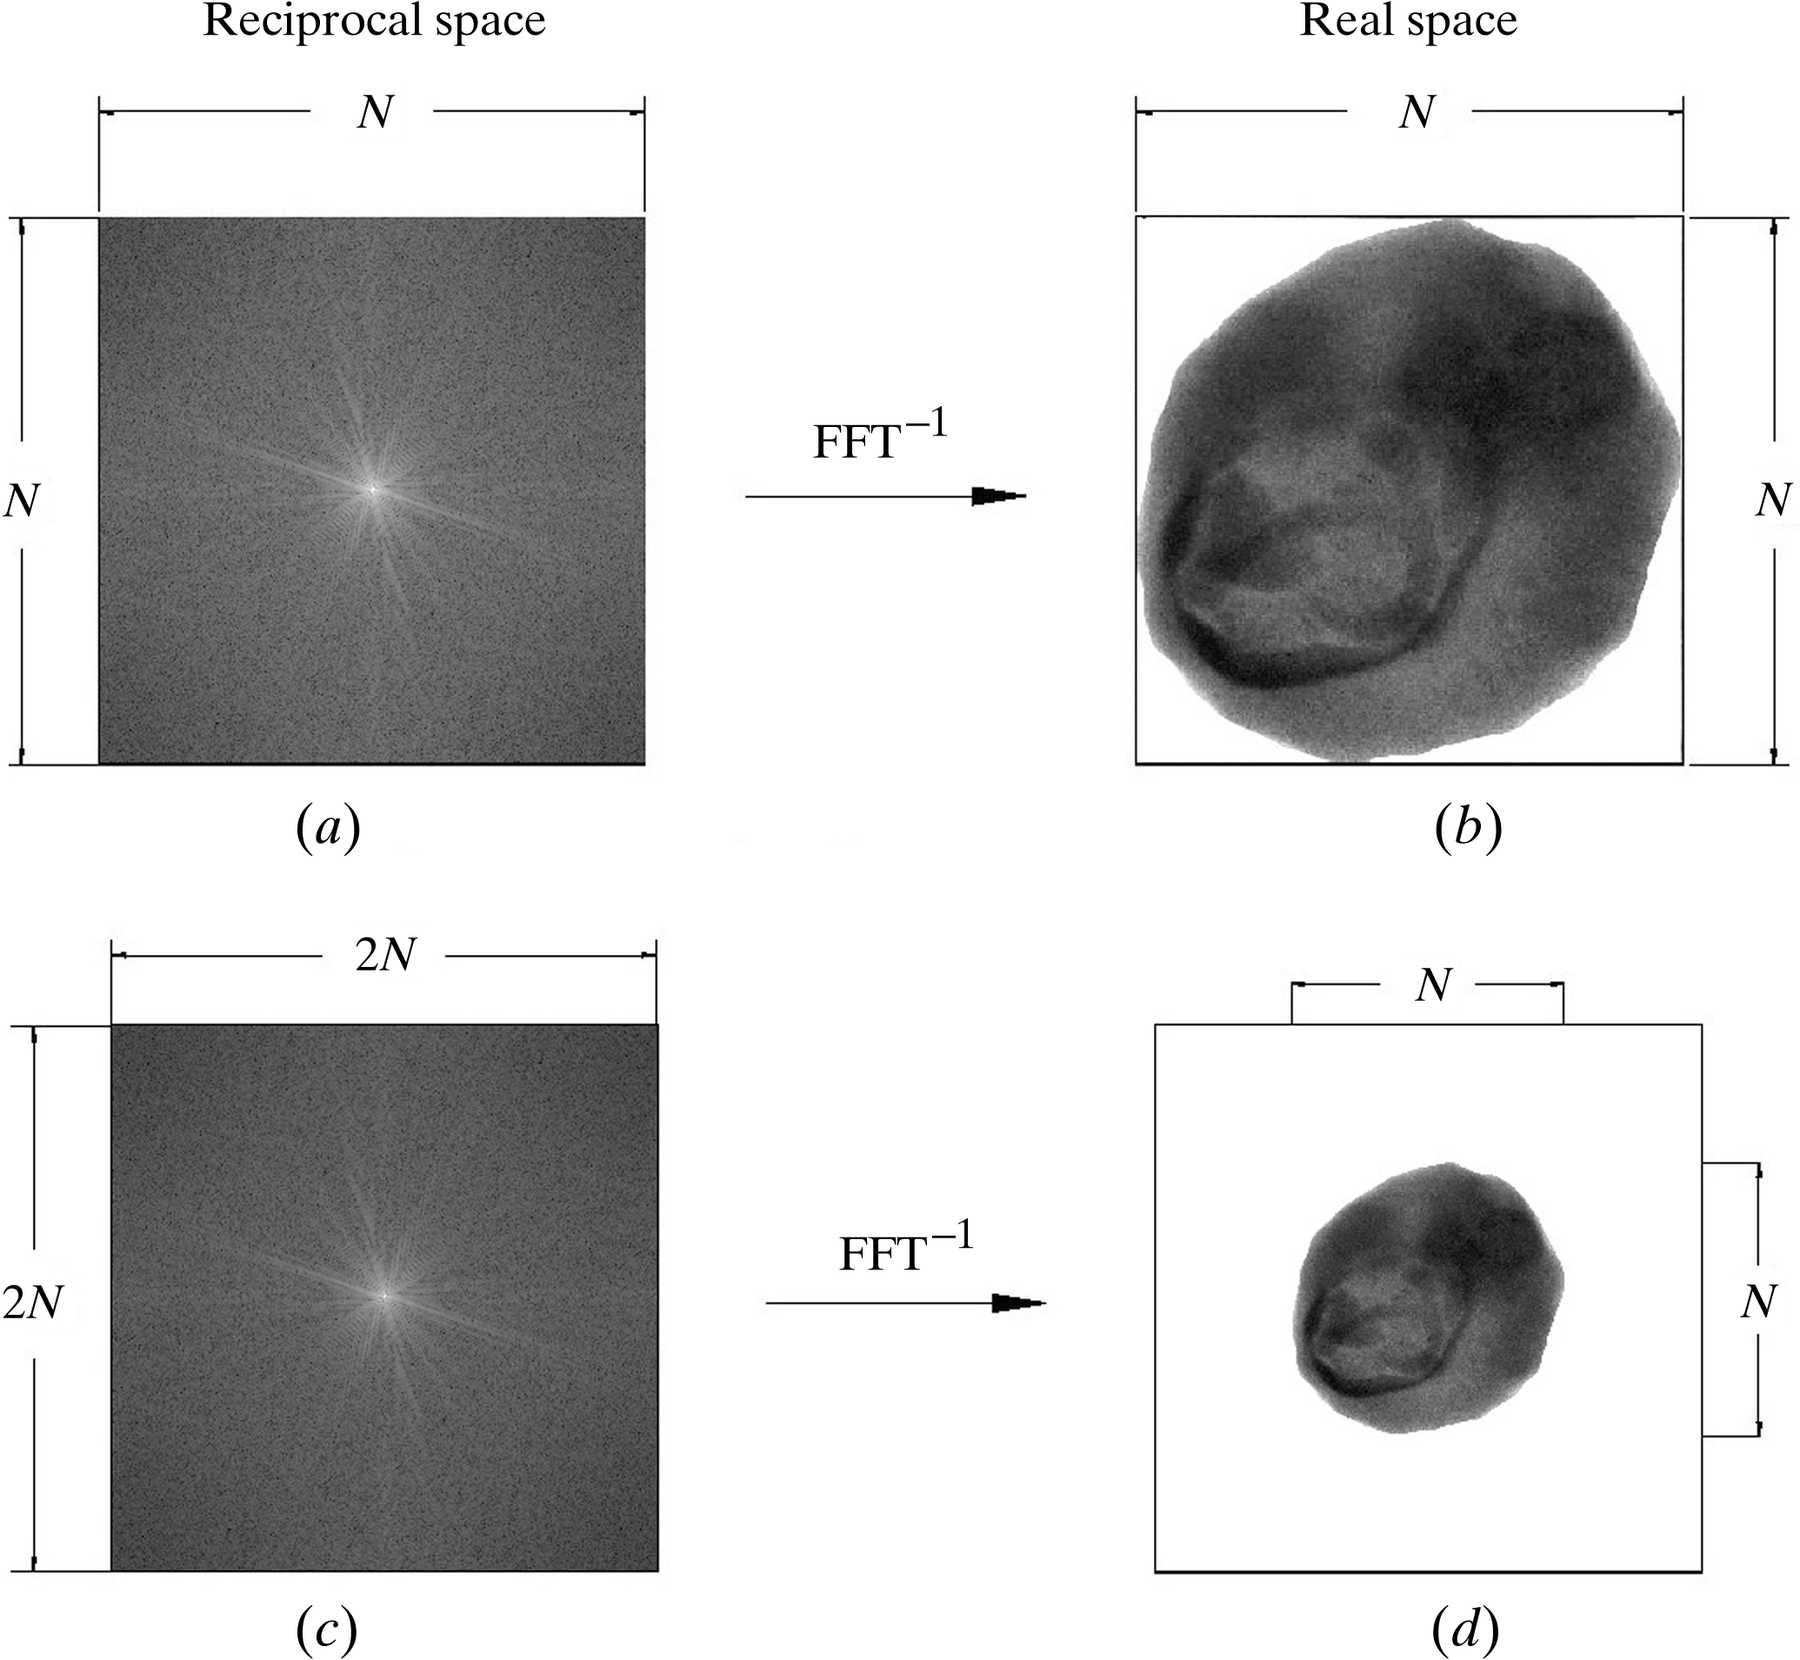
\includegraphics[height=5cm]{images/bk0084fig1mag.jpg}}
        \qquad
        \subfigure{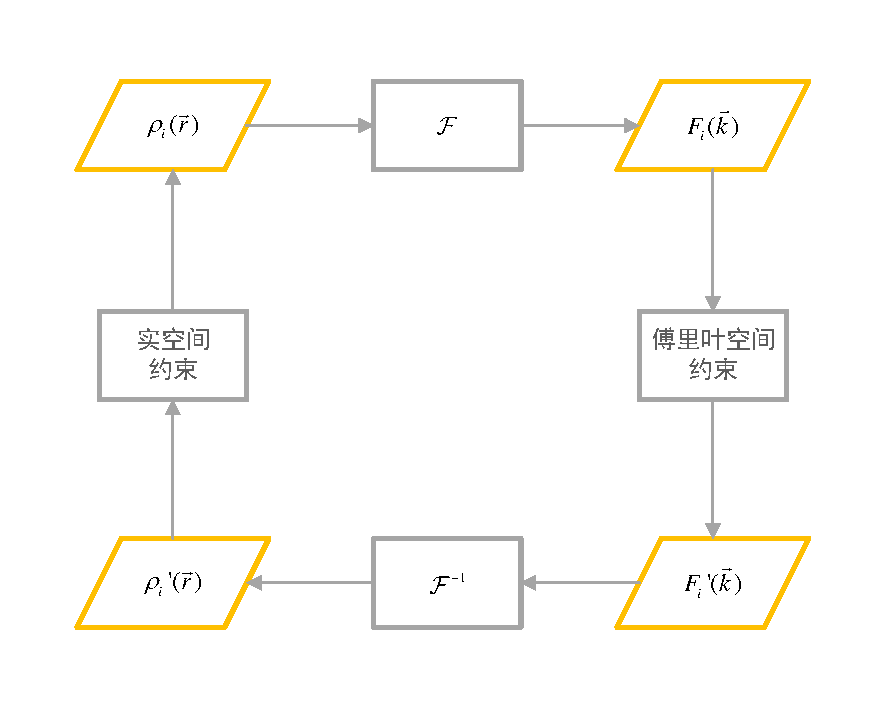
\includegraphics[height=5cm]{images/1.pdf}}
    \end{figure}
\end{frame}

\begin{frame}
    \frametitle{ER-HIO}
    \begin{figure}
        \subfigure{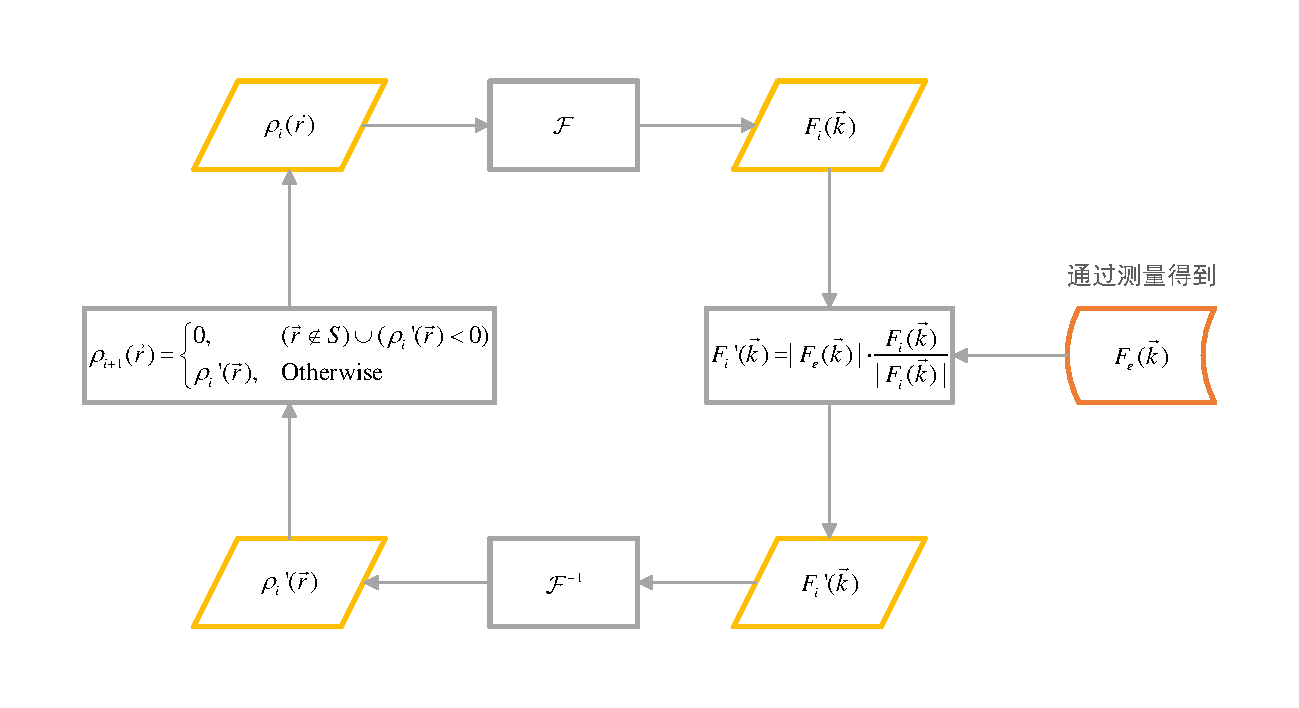
\includegraphics[height=3.6cm]{images/2.pdf}}
        \subfigure{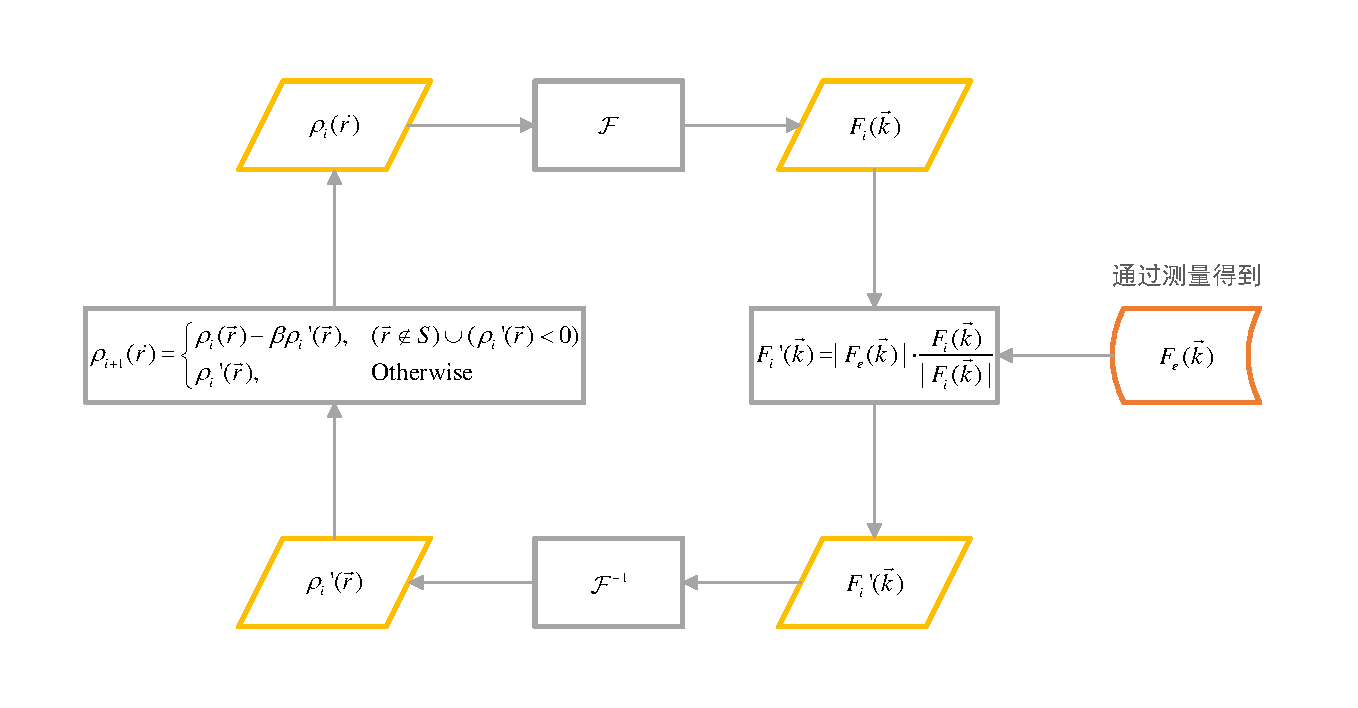
\includegraphics[height=3.6cm]{images/3.pdf}}
    \end{figure}
\end{frame}

\begin{frame}
    \frametitle{OSS}
    \begin{figure}
        \subfigure{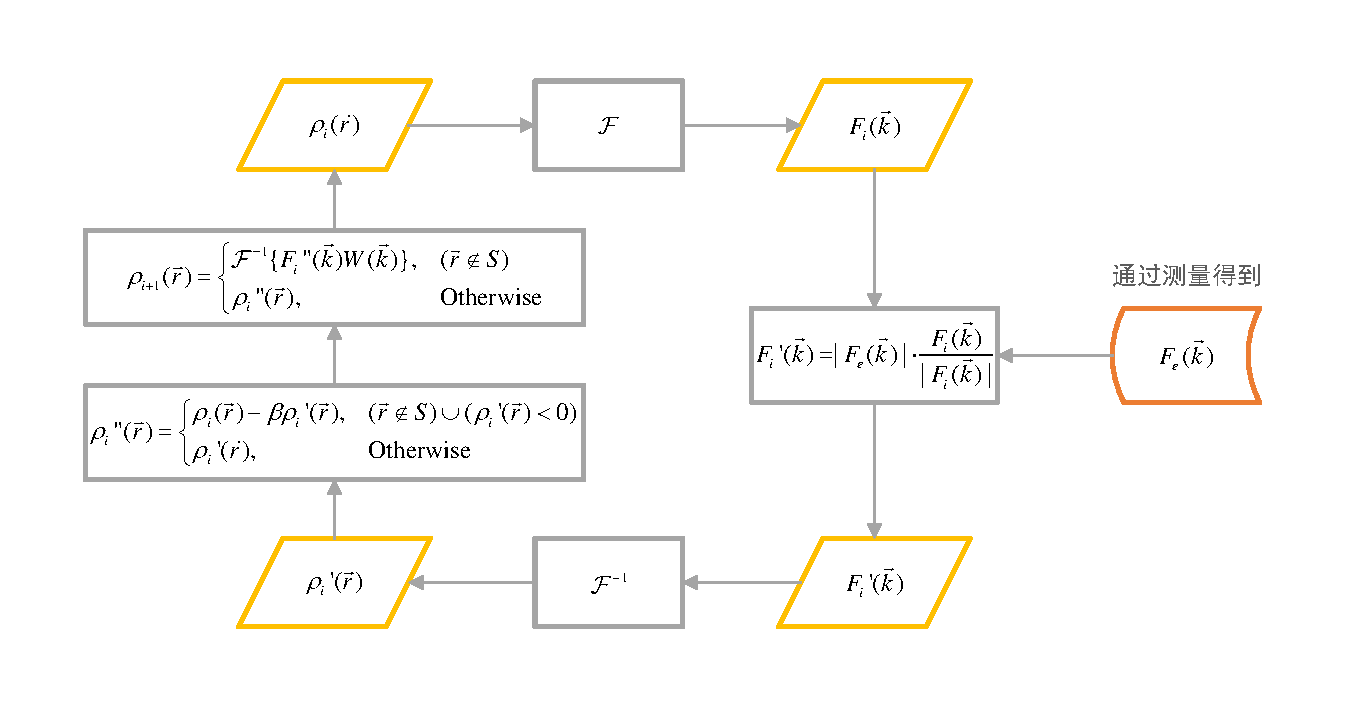
\includegraphics[height=5cm]{images/5.pdf}}
        \subfigure{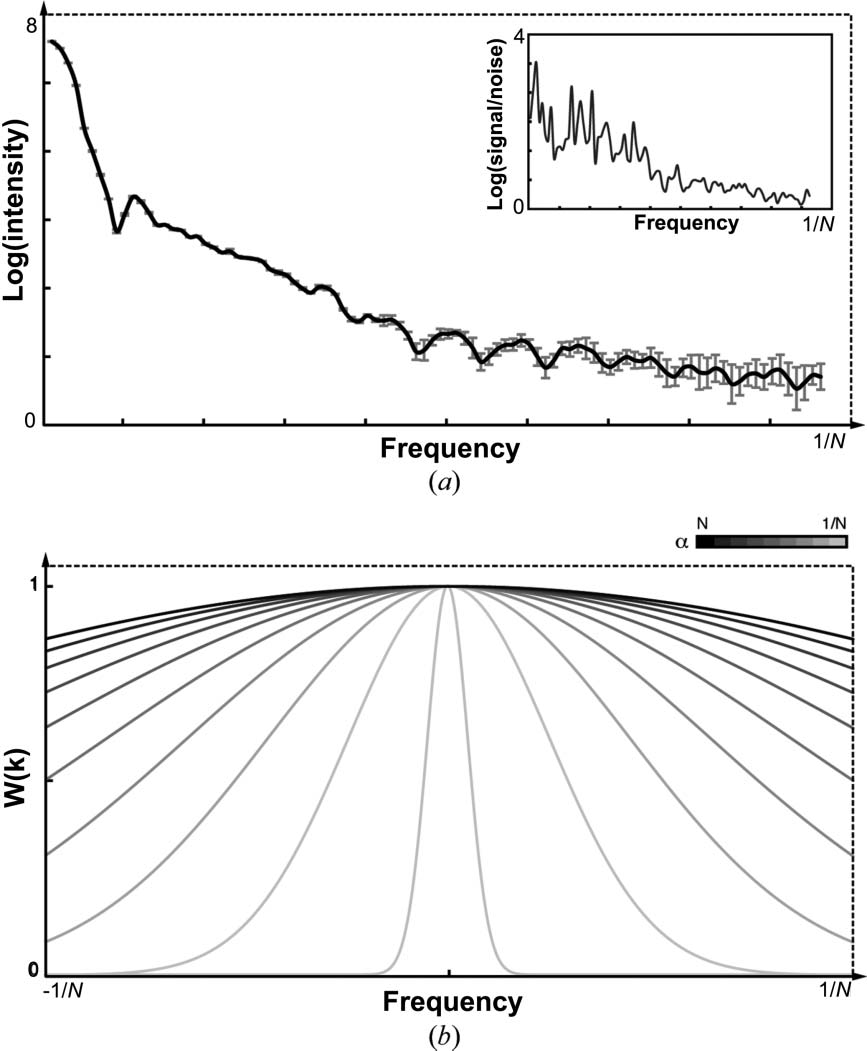
\includegraphics[height=5cm]{images/OSS_JAC_2013Oversampling smoothness-an effective algorithm.jpg}}
    \end{figure}
\end{frame}

\subsection{X-Ray Ptychography}

\begin{frame}
    \begin{figure}
        \subfigure{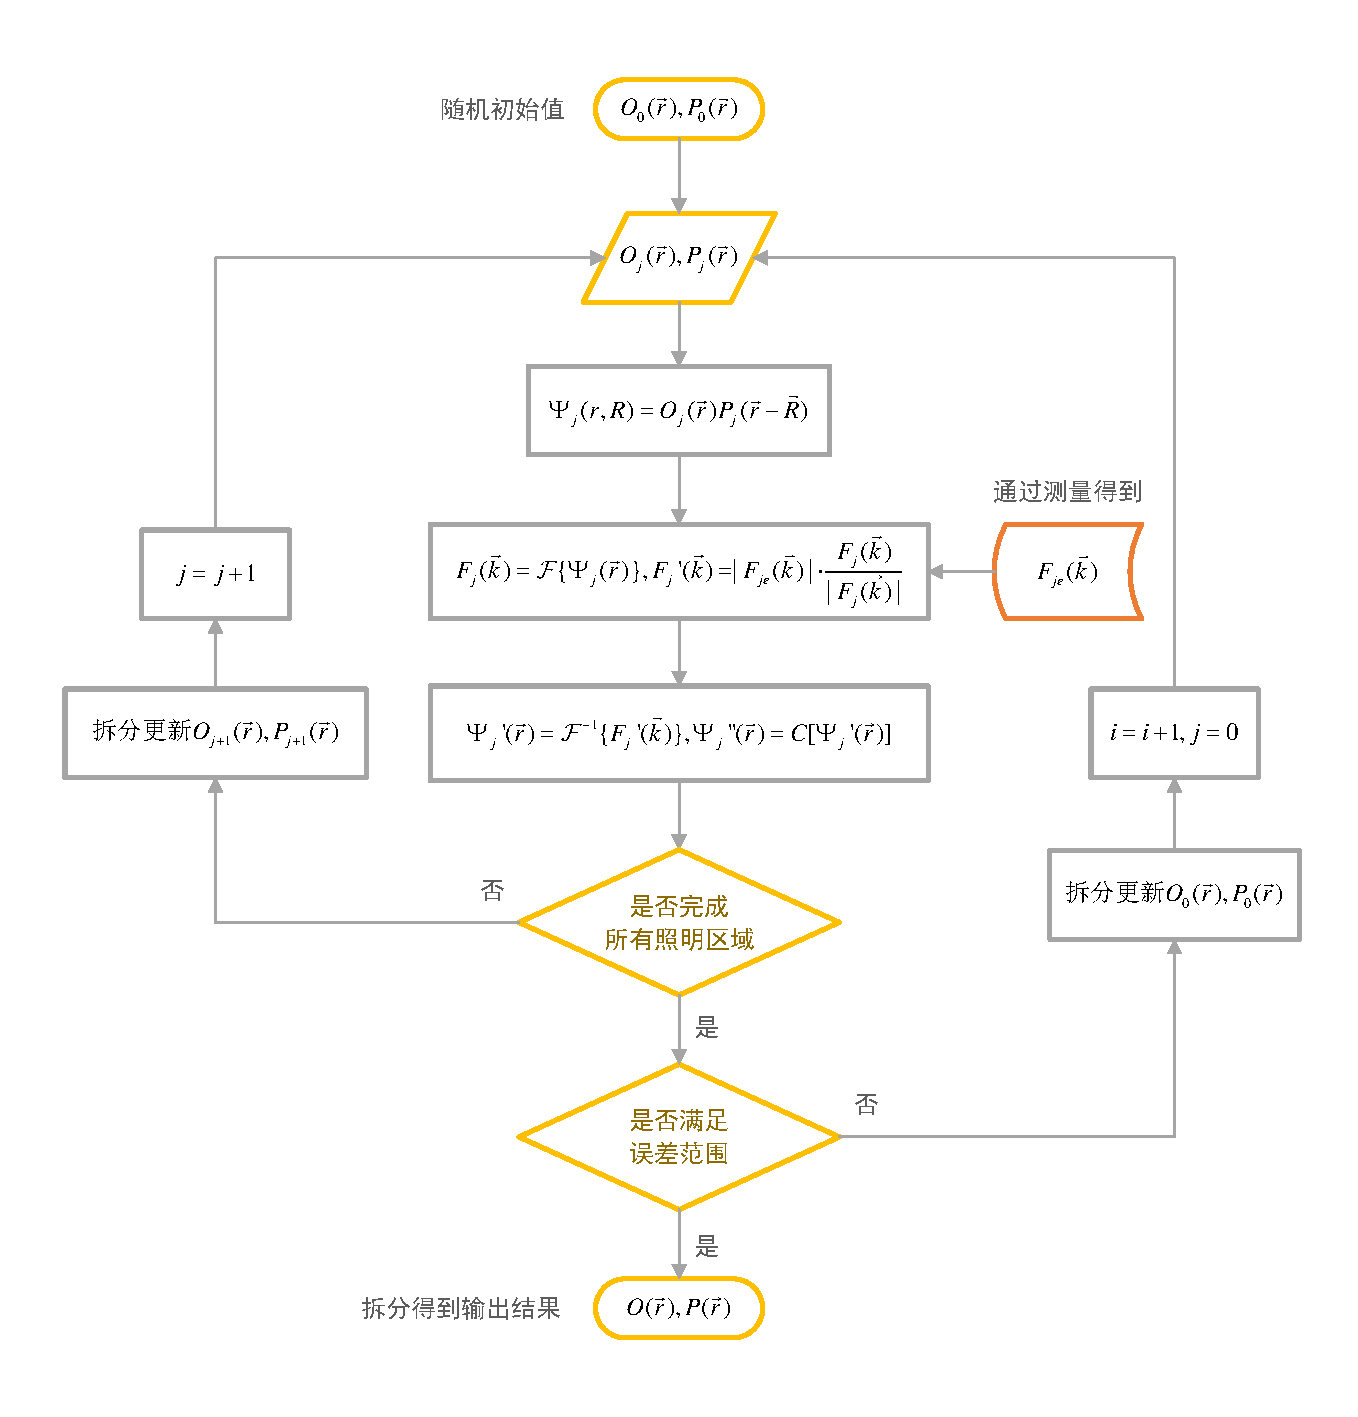
\includegraphics[height=6cm]{images/6.pdf}}
        \subfigure{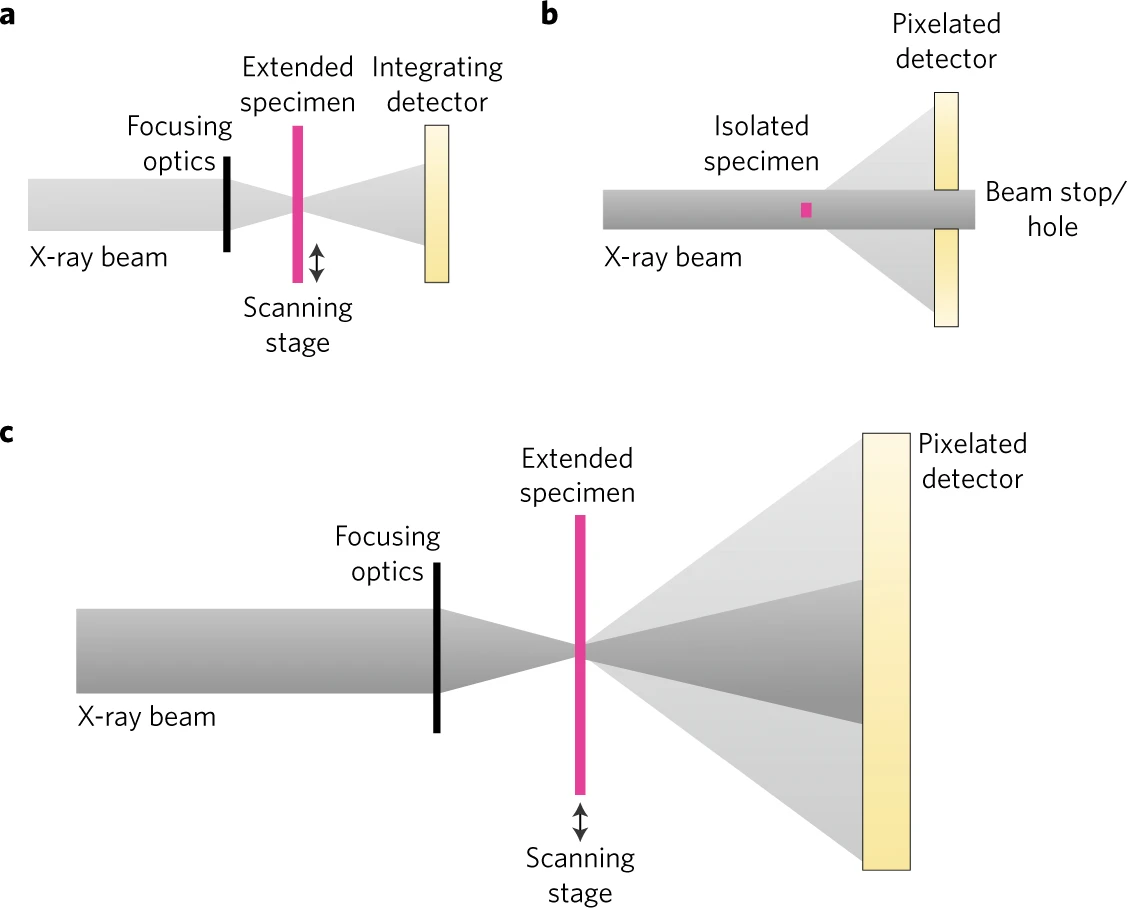
\includegraphics[height=6cm]{images/41566_2017_72_Fig1_HTML.png}}
    \end{figure}
\end{frame}

\begin{frame}
    \begin{figure}
        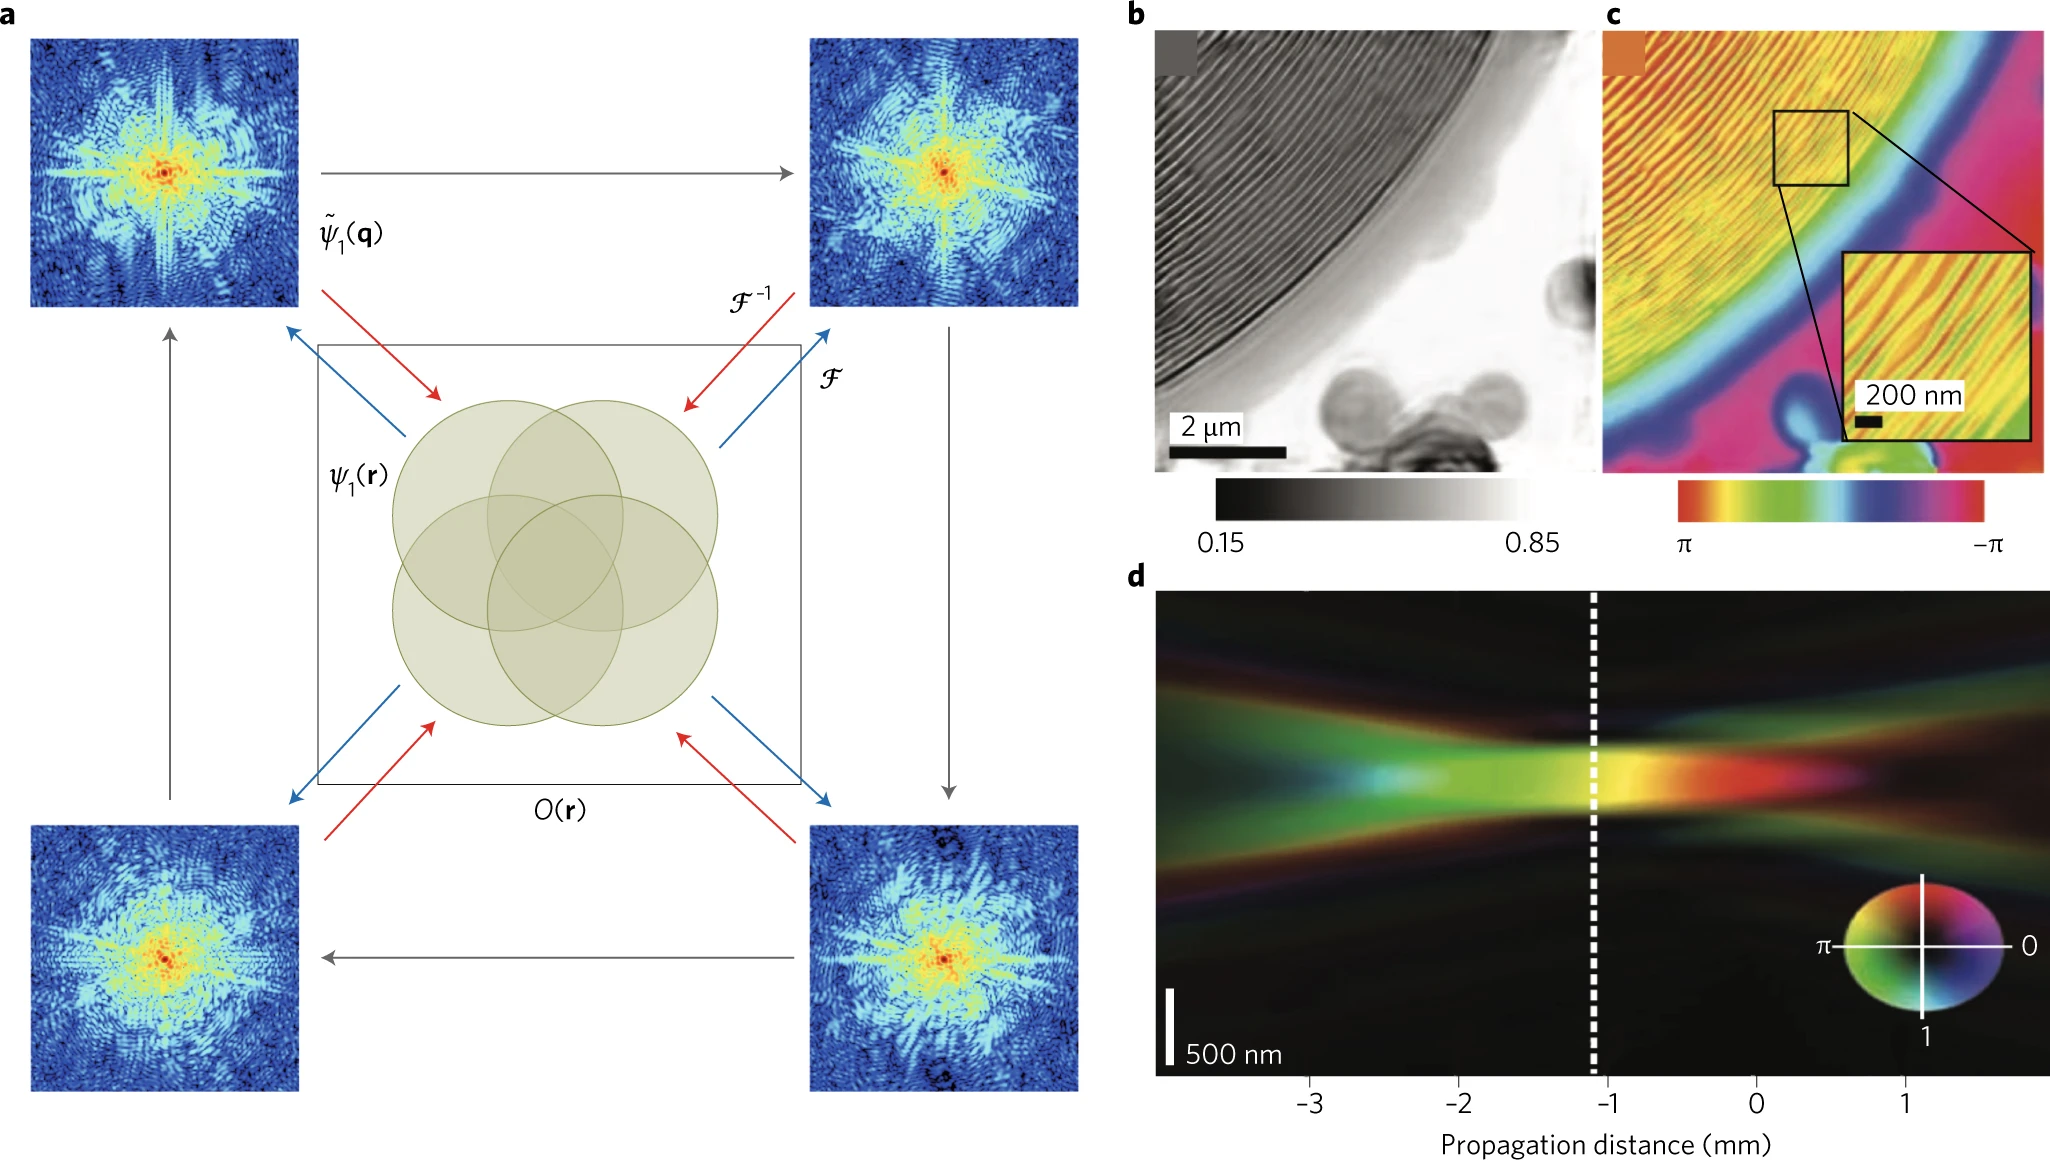
\includegraphics[height=6cm]{images/41566_2017_72_Fig2_HTML.png}
    \end{figure}
\end{frame}

\section{三维}

\subsection{傅里叶切片}

\begin{frame}
    \begin{figure}
        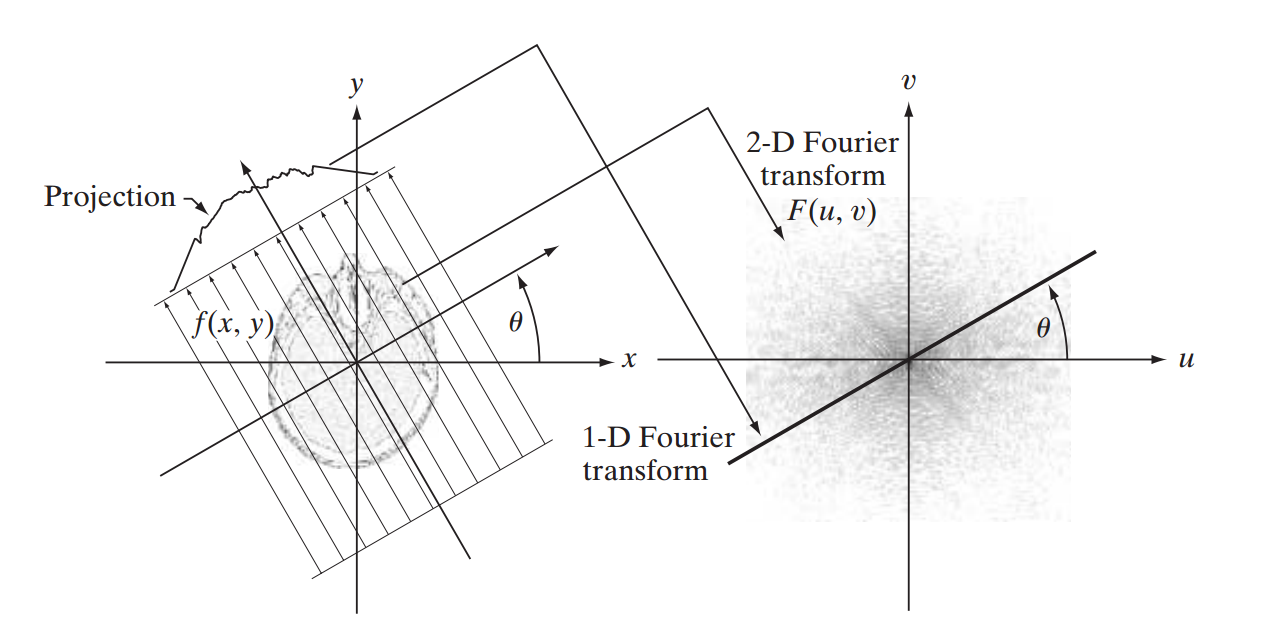
\includegraphics[height=6cm]{images/20180410092110702.png}
    \end{figure}
\end{frame}

\subsection{重建算法}

\begin{frame}
    \begin{columns}
        \begin{column}{0.4\textwidth}
            \begin{figure}
                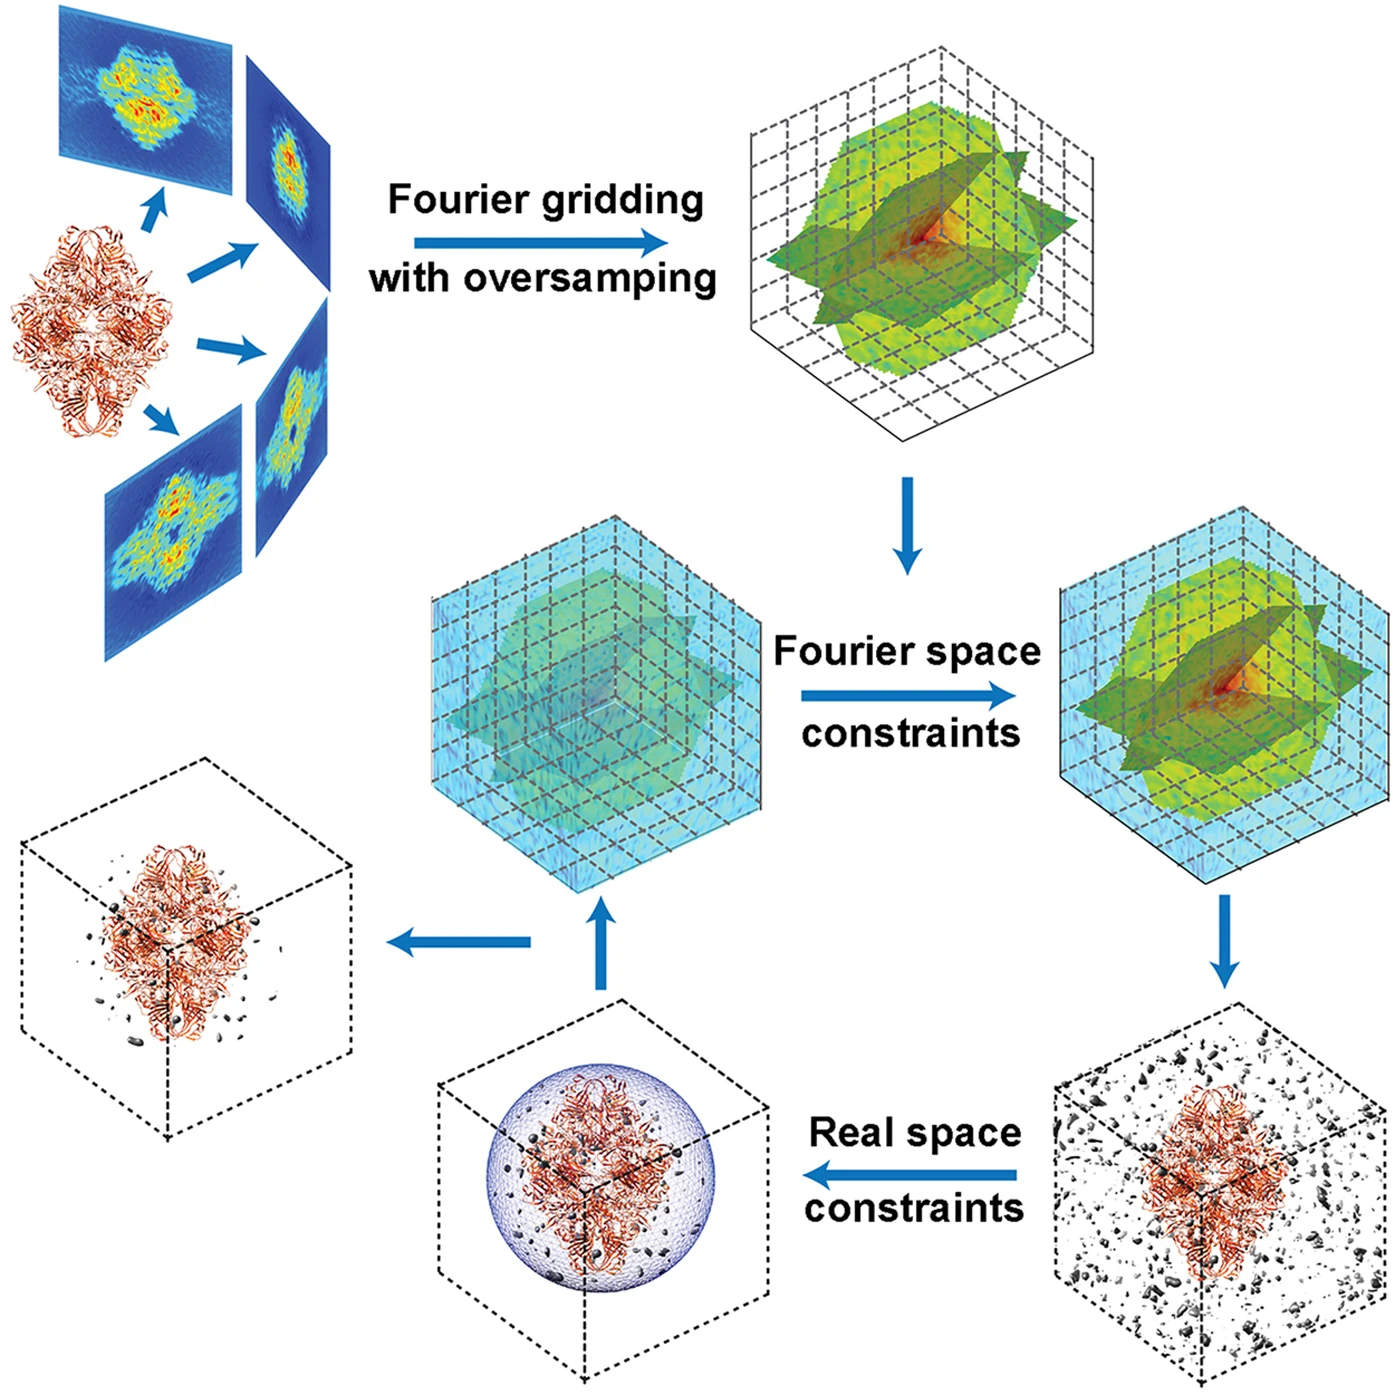
\includegraphics[height=5cm]{images/41598_2017_9847_Fig1_HTML.png}
                \caption{GENFIRE}
            \end{figure}
        \end{column}
        \begin{column}{0.6\textwidth}
            \begin{block}{其他重建算法}
                \begin{itemize}
                    \item 滤波反投影(Filtered Back Projection, FBP)
                    \item 卷积反投影(Convolution Back Projection, CBP)
                    \item 代数重构技术(Algebraic Reconstruction Technique, ART)
                \end{itemize}
            \end{block}
        \end{column}
    \end{columns}
\end{frame}

\section{实验}

\subsection{X-Ray Ptychography}

\begin{frame}
    \begin{figure}
        \subfigure{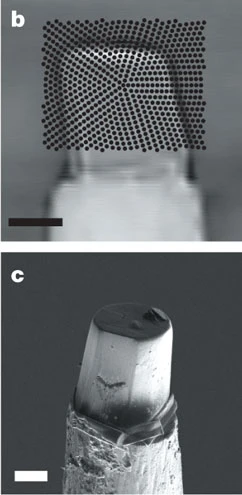
\includegraphics[height=6cm]{images/41586_2010_Article_BFnature09419_Fig1_HTML.png}}
        \qquad
        \subfigure{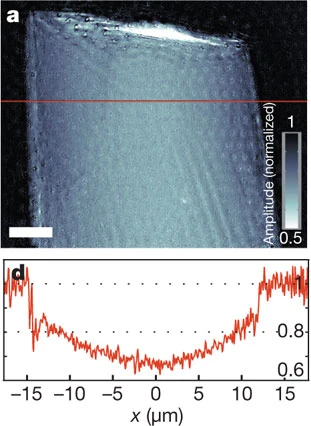
\includegraphics[height=6cm]{images/41586_2010_Article_BFnature09419_Fig2_HTML.png}}
    \end{figure}
\end{frame}

\subsection{Holler}

\begin{frame}
    \begin{figure}
        \subfigure{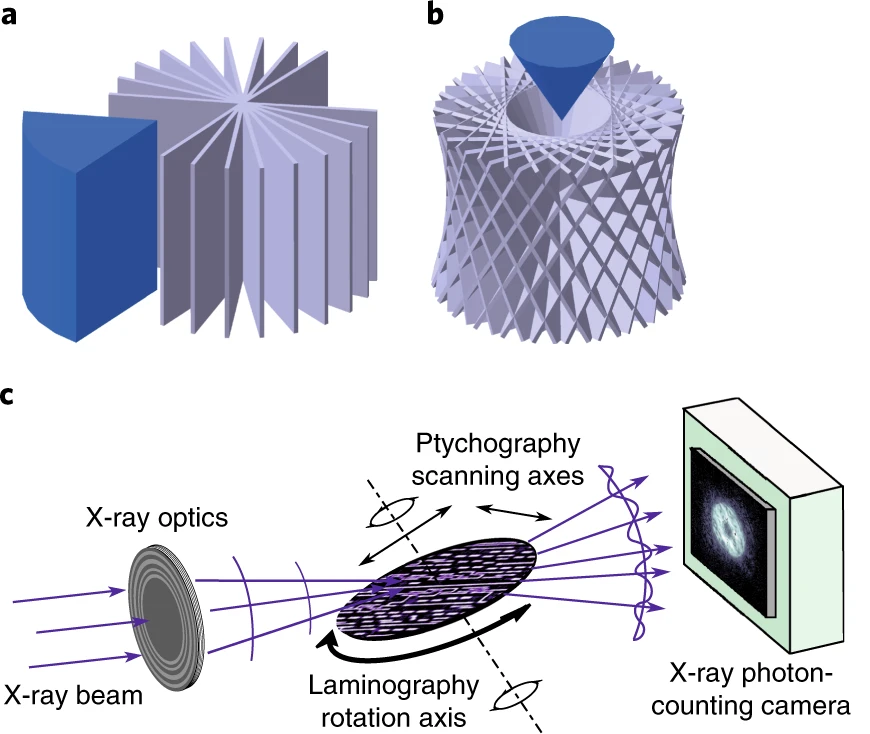
\includegraphics[height=5.8cm]{images/41928_2019_309_Fig1_HTML.png}}
        \subfigure{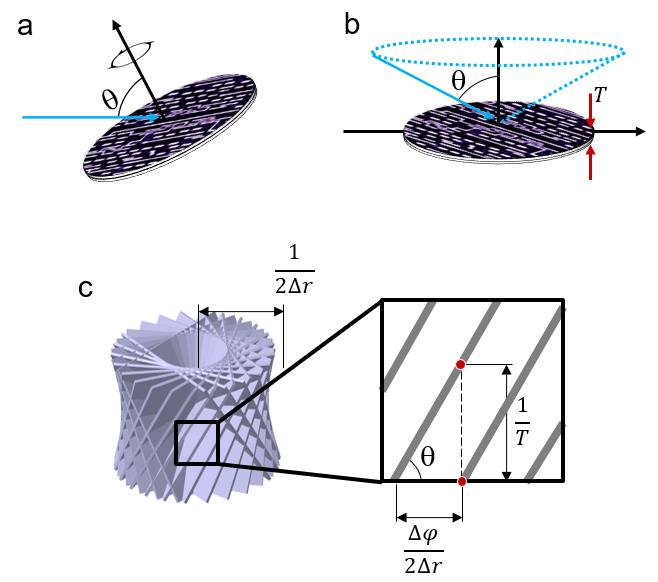
\includegraphics[height=5.8cm]{images/X.png}}
    \end{figure}
\end{frame}

\section{改进思考}

\begin{frame}
    \frametitle{二维成像}
    \begin{block}{没有实质性进展}
        \begin{itemize}
            \item 降噪算法并不理想
            \item X-Ray Ptychography可以弥补单次CDI的缺点
        \end{itemize}
    \end{block}
\end{frame}

\begin{frame}
    \frametitle{三维重建}
    \begin{block}{傅里叶网格}
        \begin{itemize}
            \item 在不同的位置网格稀疏不一,有些地方的网格无法获得精确数据的网格,只能按照未知处理。
            \item 数据密集的地方,如何最大限度的使用;测量数据。
            \item 传统的网格是均匀的,也许可以设置密度不一的网格。
        \end{itemize}
    \end{block}
\end{frame}

    \begin{frame}
        \frametitle{三维重建} 
    \begin{block}{重建算法}
        \begin{itemize}
            \item 苗老师的代码已经十分完善,且开源,提高效率只能寄托于硬件。
            \item 考虑将GENFIRE与其他较为成熟的算法进行结合,例如FBP、ART等。
        \end{itemize}
    \end{block}
\end{frame}

\end{document}